\sectionthree{Implementing a single DFA in C++}
\begin{python0}
  from solutions import * ; clear()
\end{python0}

You can actually simulate the computation
of a DFA using a programming language such as C++, Java, etc.
Let's write a C++ program to simulate this DFA:

\begin{center}
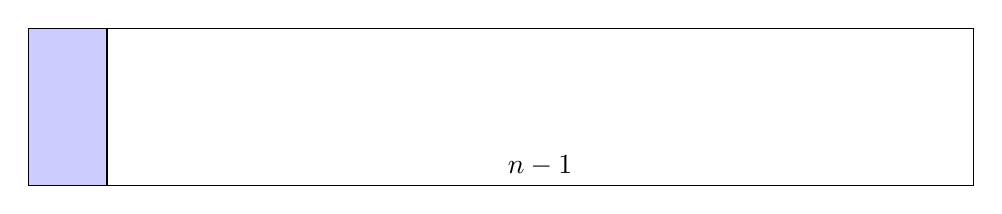
\begin{tikzpicture}

\draw (6.0, 1.0)
  node[draw, , , color=black,
       rounded corners=0cm, inner sep=0cm] {

\begin{minipage}[t][2cm]{12cm}
\mbox{}

\end{minipage}

};
\draw (0.5, 1.0)
  node[fill=blue!20!white,rounded corners=0cm,inner sep=0cm] {

\begin{minipage}[t][2cm]{1cm}
\mbox{}

\end{minipage}

};
\draw (0.5, 1.0)
  node[draw, , , color=black,
       rounded corners=0cm, inner sep=0cm] {

\begin{minipage}[t][2cm]{1cm}
\mbox{}

\end{minipage}

};
\draw (6.5, 0.25)
  node[draw=none, line width=0cm, , color=black,
       rounded corners=0cm, inner sep=0cm] {

\begin{minipage}[t][0.1cm]{0.1cm}
\mbox{}

\end{minipage}

};\draw (6.5, 0.25) node[color=black] {$n - 1$};
\end{tikzpicture}

\end{center}



Here's the program:
\begin{Verbatim}[frame=single, fontsize=\small]
#include <iostream>
#include <string>

int main()
{
    std::string x;
    std::cin >> x;

    int state = 0;
    std::cout << 'q' << state << ", ";
    for (int i = 0; i < x.length(); i++)
    {
        char c = x[i];
        switch (state)
        {
            case 0:
                if (c == 'a') state = 0;
                else if (c == 'b') state = 1;
                break;
            case 1:
                if (c == 'a') state = 0;
                else if (c == 'b') state = 2;
                break;
            case 2:
                break;
        } 
        std::cout << 'q' << state << ", ";
    }
   
    std::cout << (state == 2 ? "" : "not ")
              << "accepted\n";
    return 0;
}
\end{Verbatim}
Study it carefully.

In the program, I'm using integer values to denote states.

For this program, the states of a computation is shown as well as whether is
is accepted or not.

%-*-latex-*-

\begin{ex} 
  \label{ex:prob-00}
  \tinysidebar{\debug{exercises/{disc-prob-28/question.tex}}}

  \solutionlink{sol:prob-00}
  \qed
\end{ex} 
\begin{python0}
from solutions import *
add(label="ex:prob-00",
    srcfilename='exercises/discrete-probability/prob-00/answer.tex') 
\end{python0}


(ANOTHER SECTION)

Of course the above program hardcoded lots of information.
This means that it's impossible to run a different DFA, you would have to
write another program.
It's better to have a general library for creating DFAs.

To implement such as class, we have to look at the
formal definition of a DFA.
A DFA $M$ is made up of
\begin{enumerate}[label=\textnormal{(\alph*)},itemsep=0pt,nosep,noitemsep,partopsep=0pt,topsep=0pt,parsep=0pt]
  \li $\Sigma$ is a finite set
  \li $Q$ is a finite set
  \li $q_0$ is an element in $Q$
  \li $F$ is a subset of $Q$
  \li $\delta: Q \times \Sigma \rightarrow Q$ is a function 
\end{enumerate}
The definition makes it clear that we need to implement
sets and functions.

